\section{Annealed Stein variational gradient descent}\label{sec:asvgd} 




\captionsetup[subfigure]{labelformat=empty}
\begin{figure}[t!]
    \centering 
\begin{subfigure}[b]{.48\textwidth} 
    \scalebox{1}{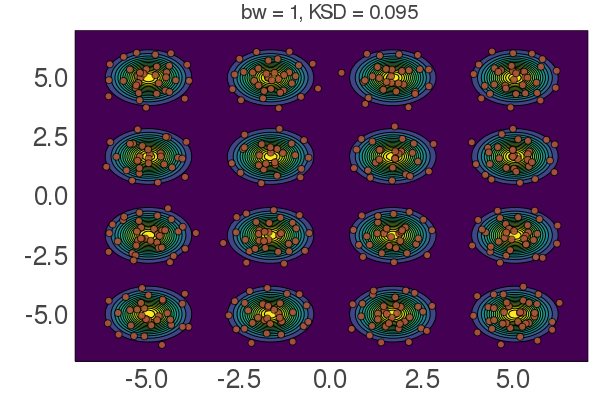
\includegraphics[width=\textwidth]{figures/bw1.png}}
    \caption{(a)\label{fig:bw1}}
\end{subfigure}
\hfill
\centering
\begin{subfigure}[b]{0.48\textwidth}
    \scalebox{1}{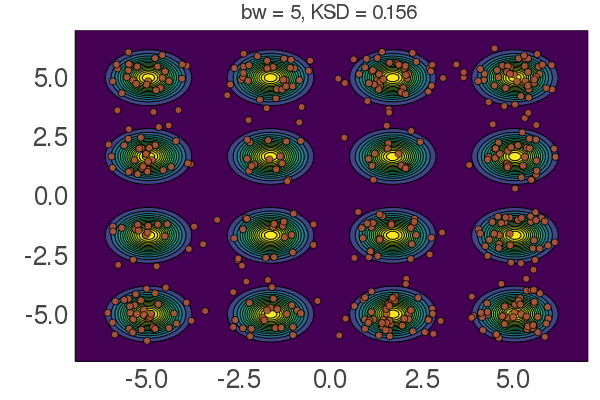
\includegraphics[width=\textwidth]{figures/bw5.png}}
    \caption{(b)\label{fig:bw5}}
\end{subfigure}
\hfill
\centering
\begin{subfigure}[b]{0.48\textwidth}
    \scalebox{1}{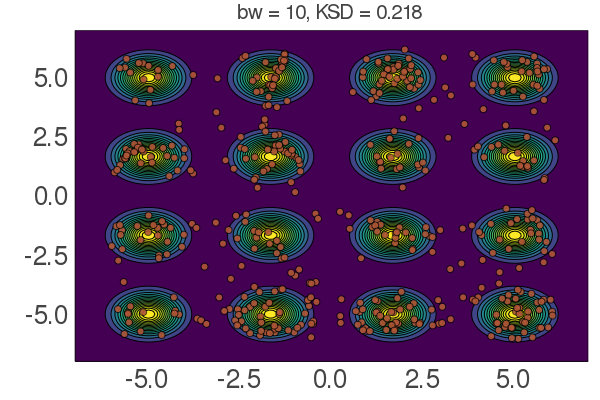
\includegraphics[width=\textwidth]{figures/bw10.png}}
    \caption{(c)\label{fig:bw10}}
\end{subfigure}
\hfill
\centering
\begin{subfigure}[b]{0.48\textwidth}
    \scalebox{1}{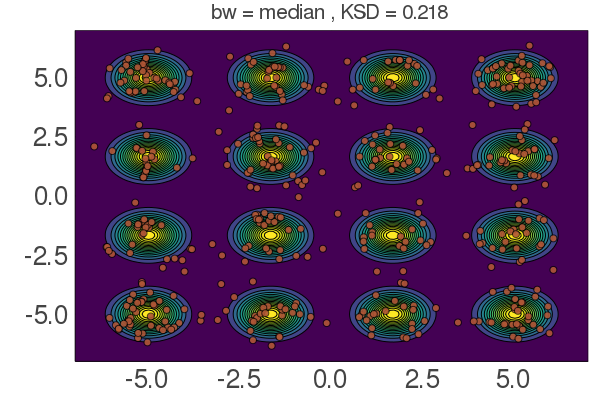
\includegraphics[width=\textwidth]{figures/bwmed.png}}
    \caption{(d)\label{fig:bwmed}}
\end{subfigure}

\caption{Comparison of A-SVGD on the synthetic Gaussian mixture with 16 components across different bandwidth. The KSDs are estimated using the same kernel.}
\label{fig:BW}
\end{figure}








\captionsetup[subfigure]{labelformat=empty}
\begin{figure}[t!]
    \centering 
\begin{subfigure}[b]{.48\textwidth} 
    \scalebox{1}{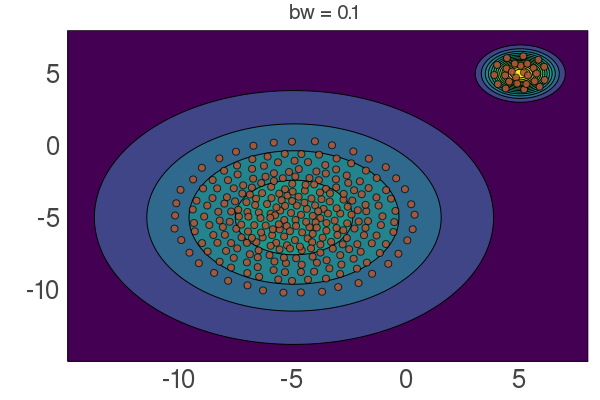
\includegraphics[width=\textwidth]{figures/bwsmall.png}}
    \caption{(a)\label{fig:bwsmall}}
\end{subfigure}
\hfill
\centering
\begin{subfigure}[b]{0.48\textwidth}
    \scalebox{1}{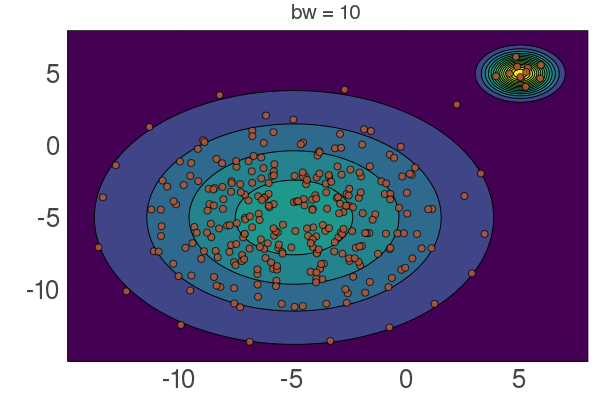
\includegraphics[width=\textwidth]{figures/bwlarge.png}}
    \caption{(b)\label{fig:bwlarge}}
\end{subfigure}
\hfill
\centering
\begin{subfigure}[b]{0.48\textwidth}
    \scalebox{1}{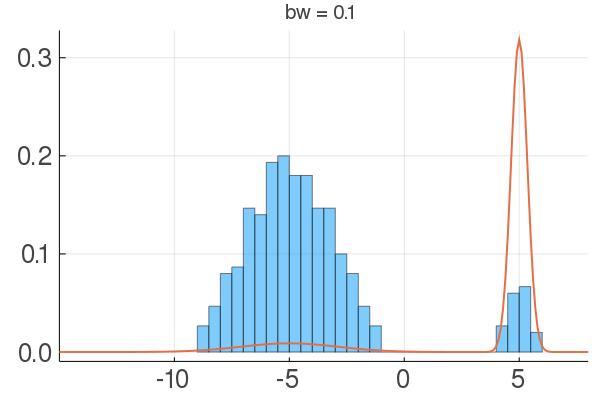
\includegraphics[width=\textwidth]{figures/slice_small.png}}
    \caption{(c)\label{fig:slice_small}}
\end{subfigure}
\hfill
\centering
\begin{subfigure}[b]{0.48\textwidth}
    \scalebox{1}{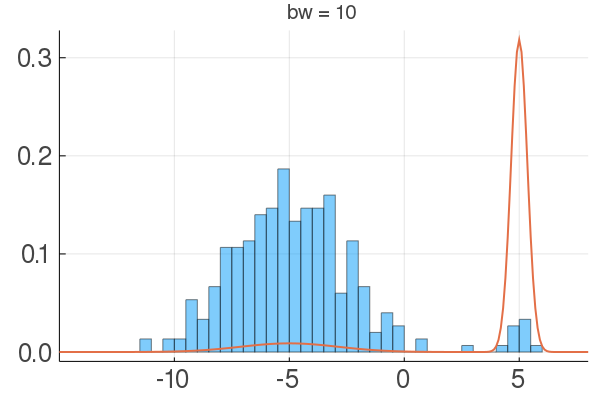
\includegraphics[width=\textwidth]{figures/slice_large.png}}
    \caption{(d)\label{fig:slice_large}}
\end{subfigure}


\caption{Comparison of A-SVGD on a 2-component Gaussian mixture with different bandwidth. \cref{fig:bwsmall,fig:bwlarge} show scatter plots of particles at the last iteration. \cref{fig:slice_small,fig:slice_large} show histograms of the particles by projecting the locations to the line $y = x$, where the orange curve denotes the density of Gaussian mixture along the slice $y = x$.}
\label{fig:differentBW}
\end{figure}


\begin{figure}[t!]
    
\end{figure}


\captionsetup[subfigure]{labelformat=empty}
\begin{figure}[t!]
    \centering 
\begin{subfigure}[b]{.48\textwidth} 
    \scalebox{1}{\includegraphics[width=\textwidth]{figures/mixGauss.png}}
    \caption{(a) \label{fig:bwlocal}}
\end{subfigure}
\hfill
\centering
\begin{subfigure}[b]{0.48\textwidth}
    \scalebox{1}{\includegraphics[width=\textwidth]{figures/slice_gauss.png}}
    \caption{(b)\label{fig:slicelocal}}
\end{subfigure}

\caption{A-SVGD with localized Gaussian kernel on a 2-component Gaussian mixture.}
\label{fig:localbw}
\end{figure}


\captionsetup[subfigure]{labelformat=empty}
\begin{figure}[t!]
    \centering 
\begin{subfigure}[b]{.48\textwidth} 
    \scalebox{1}{\includegraphics[width=\textwidth]{figures/grid_gs.png}}
    \caption{(a) $\{x_i^{(0)}\}_{i = 1}^{500} \distiid \distNorm(0\ind, 0.25I)$  \label{fig:bwlocal}}
\end{subfigure}
\hfill
\centering
\begin{subfigure}[b]{0.48\textwidth}
    \scalebox{1}{\includegraphics[width=\textwidth]{figures/grid_gs10.png}}
    \caption{(b) $\{x_i^{(0)}\}_{i = 1}^{500} \distiid \distNorm(10\ind, 0.25I)$ \label{fig:slicelocal}}
\end{subfigure}

\caption{A-SVGD with localized Gaussian kernel on a $4 \times 4$ Gaussian mixture.}
\label{fig:gridlocal}
\end{figure}

A key limitation of SVGD is the mixing issue when the target
distribution $p(x)$ has multiple modes, where the
particles collapse at a particular mode and fail
to explore other high density regions. This is also known
as the \emph{mode collapse} phenomenon \citep{zhuo2018message,d2021annealed}
and appears often when the modes are distant from each other. This problem tends to be more severe in high-dimensional settings, but can
also be observed on a simple 2D Gaussian mixture target. 
In this section, we provide a brief introduction of the annealed SVGD
(A-SVGD), which is developed to address the mixing issue
\citep{d2021annealed}, and use a few synthetic examples to identify a key
limitation of the current work. The design of the synthetic example aims to
understand the influence of the kernel bandwidth on the behaviour of SVGD or
A-SVGD and help us to build the intuition of picking a proper value. The
experiments performed in this report use the RMSprop update rule
\cref{eq:rms}. We run both SVGD and A-SVGD with standard RBF kernel for
$1000$ iterations under a constant learning rate $\gamma_k = 0.1$.



We start with the development of A-SVGD. Considering the updates
\cref{eq:svgd}, the optimal descent direction $ \hat{\phi}^{\star}(x)$ for
the particle $x$ includes two parts: the driving force that moves the
particle to a high density region of $p(x)$, and a repulsion that prevents
the particles collapsing together. The specific derivation is as follows,
\[
    \hat{\phi}_k^{\star}(x)=\frac{1}{n} \sum_{j=1}^{n}\left[\underbrace{\kappa\left(x_{j}^{(k)}, x\right) \nabla \log p\left(x_{j}^{(k)}\right)}_{\text {driving force }}+\underbrace{\nabla_{x_{j}^{(k)}} \kappa\left(x_{j}^{(k)}, x\right)}_{\text {repulsion }}\right].
\]
When mode collapse occurs, particles produced by SVGD are trapped at some
region and fail to explore the full support of $p(x)$. This often happens
when the driving force dominates the repulsion. An intuitive solution is to
boost the repulsion or scale down the driving force to enable a wider spread
of the particles.
\citet{d2021annealed} follows this intuition and modify the descent direction
by introducing an annealing term $\alpha(k) \in [0, 1]$:
\[\label{eq:asvgd}
    \hat{\phi}_{\alpha_k}\left(x\right) = \frac{1}{n} \sum_{j=1}^{n}\left[ \alpha(k)\kappa\left(x_{j}^{(k)}, x\right) \nabla \log p\left(x_{j}^{(k)}\right)+ \nabla_{x_{j}^{(k)}} \kappa\left(x_{j}^{(k)}, x\right)\right].
\]
In particular, the authors suggest using a cyclical annealing schedule, i.e., 
\[\label{eq:anneal_sched}
    \alpha(k)=\left(\frac{\bmod (k, K / C)}{K / C}\right)^{p},
\]
where $K$ is the total number of iterations, $C$ is the number of cycles, and
$p > 0$ is an exponent factor that controls the speed of the transition
between two phases. As demonstrated in \cref{fig:acsched}, smaller $p$
corresponds to a shorter period of the exploratory phase. For the two synthetic Gaussian mixture examples of this section, we set $ p = 1$ and $C = 2$ for A-SVGD. 

Now we compare the performance of A-SVGD and SVGD on a synthetic Gaussian
mixture (\cref{fig:SVGD_ASVGD}). The target distribution is a 2D mixture of
$16$ Gaussian component with means equally distributed on a $4 \times 4$ grid
with identical covariance $0.25I$. We consider two different initialization
particles: \cref{fig:T0_rms,fig:T0_rms_anneal} are initialized with $500$
\iid samples from $\distNorm(0, 0.25I)$;
\cref{fig:T10_rms,fig:T10_rms_anneal} are initialized with $500$ \iid samples
from $\distNorm(10, 0.25I)$. In this example, we use RBF kernel with 
$h =0.5$. Note that in both initialization schemes, A-SVGD is able to explore all
the modes while all the particles produced by SVGD collapse at the components
close by the initialization. Comparing
\cref{fig:T0_rms_anneal,fig:T10_rms_anneal}, one may notice that the
performance of A-SVGD still depend on the location of the initial particles.

\subsection{Bandwidth selection} \label{sec:bwselection}

Although A-SVGD manages to mix well, its performance relies heavily on a
good choice of kernel bandwidth. Generally, to optimize the performance of SVGD and its variants, one must tune the kernel bandwidth. The original paper \citep{liu2016stein} suggests using the median trick for the typical RBF kernel,
\[
   \kappa(x, x') = \exp(-\frac{1}{h} \|x - x'\|^2). 
\]
The bandwidth is selected based on the median of the pairwise Euclidean distances between the current particles, i.e., $h=\operatorname{med}^{2} / \log n$, where $\operatorname{med}$ is the median of the Euclidean distances. This procedure will update the bandwidth automatically at each iteration and works generally well for unimodal target distribution. However, we will show that the median trick can be problematic when the local geometry of $\log p$ is complicated.

\cref{fig:BW} present the results of A-SVGD
on the same target across $4$ different kernel bandwidth: $h = 1, 5, 10$ and
the median heuristic (will be introduced in \cref{sec:bw}). The initial
particles are $500$ \iid samples from $\distNorm(0, 0.25I)$. We find that as
$h$ increases (not even a large amount), the convergence of A-SVGD gets
ruined. Moreover, the median trick suggested by \citet{liu2016stein}
completely fails. For quantitative characterization of the sample qualities,
we compute the kernelized Stein discrepancy,which shows a decreasing sample
quality as $h$ increases. The key reason is that as the annealing schedule
enables the points to traverse over different modes in the exploratory phase,
the particles need to quickly converge to the high-density region around them
in the converging phase. As we mentioned previously, the driving force will
push the samples along the $\nabla \log p(x)$. However, the driving force is
a weighted summation of $\nabla \log p(x_i), i=1, 2, \dots, n$ and weights
are controlled by the kernel. Adopting a large bandwidth tends to include
misleading information from the particles that converge to other modes.


Even though the previous example prefers a smaller bandwidth, it does not
mean that smaller $h$ is always better. We then create a pathological yet simple example such that
neither small nor large bandwidth is satisfying.
Considering a two-component Gaussian mixture:
\[
\frac{1}{2}\distNorm\left( -5 \ind, 9I \right)  + \frac{1}{2}\distNorm\left( 5\ind, 0.25I \right).
\]
\cref{fig:differentBW} display the results of A-SVGD with $300$ initial
particles sampled from $\distNorm(0\ind, 25I )$ using different kernel
bandwidth $h = 0.1, 10$. With small $h$, particles located in the wide
Gaussian component are overly contracted; with large $h$, almost all
particles converge to the wide mode.
This is essentially due to the fact that the curvature of the local basin of
two gaussian components is quite different. When using a wide kernel
bandwidth, the driving force of those particles around the narrow Gaussian
component is significantly influenced by gradient information $\log p(x)$ of
the particles that are far away. As most particles are trapped in the wider
Gaussian component, the driving force tends to point to the wide mode. Also,
a large bandwidth leads to a stronger repulsion, which encourages the spread
of particles. On the contrary, with small bandwidth---as shown in
\cref{fig:bwsmall,fig:slice_small}---although the peaky Gaussian absorbs more
particles, a weaker repulsion makes the particles collapsing together and 
underestimate the variance of the wide Gaussian.
This hints at an important fact that using a universal kernel bandwidth for
all particles is not ideal, and we should use different kernel bandwidths
when updating each of the particles depending on its local basin of $\nabla
\log p(x)$. In the next section, we propose a localized Gaussian kernel  scheme that adaptively learns an anisotropic Gaussian kernel for each particle.




\section{Localized Gaussian kernel} \label{sec:bw}

With the intuition obtained in the last section, we suggest using different
bandwidth values for each particle and updates the bandwidth adaptively
across the iteration. The goal of this section is to design an adaptive
procedure that learns a proper kernel bandwidth for each particle
automatically. As illustrated in \cref{fig:differentBW}, a careful choice of
kernel bandwidth is necessary when the target distribution has multiple modes
and one might consider using different bandwidth values at a different
location. Intuitively, a proper choice of the bandwidth should reflect the
local geometry of $\log p(x)$---the curvature of $\log p(x)$---which includes
information of the Hessian $\nabla^2 \log p(x)$.

To generalize this idea, we consider the anisotropic Gaussian kernel with covariance $\Sigma$---a positive definite matrix,
\[
\kappa(x, x'; \Sigma) = \exp\left(-\frac{1}{2}(x - x')^T \Sigma^{-1}(x)(x- x')  \right).  
\]
Note that this anisotropic Gaussian kernel is \emph{localized} as its covariance $\Sigma$ depends on $x$. 
Intuitively, $\Sigma^{-1}$ serves as a scaling matrix to the distance between particles and induces a deformed geometry structure in the particle space, which directly affects the gradient averaging when moving each particle and the repulsion among particles.  To align with our intuition and previous synthetic experiments in \cref{sec:asvgd}, we want the particles are more influenced by neighbouring particles when the curvature is huge and more spread when the local curvature is small. Therefore propose to set $\Sigma^{-1}$ to $\text{abs}\left( \diag \left(\nabla^2 \log p(x) \right)^{-1}\right)$. We use the absolute value because the diagonal element of $\nabla^2 \log p(x)$ can be negative if $p$ is not log-concave. The complete procedure of A-SVGD
using adaptive local bandwidth is described in \cref{alg:ASVGD_bw}.

% \bnprop
% theoreticl justification for gaussian target
% \enprop



With other settings fixed, we apply \cref{alg:ASVGD_bw} to the previous two
synthetic examples. As demonstrated in \cref{fig:localbw}, by using the local
bandwidth, the samples in the wide component correctly characterize its
variance and there is a certain amount of samples concentrate at the peak
mode. This combines the advantages of both small $h$ and large $h$. And for
the 16-component Gaussian example, as shown in
\cref{fig:gridlocal}, A-SVGD using localized kernel effectively explores all
the Gaussian component regardless of the initial particles; which even
outperforms A-SVGD with hand-tuned bandwidth; and importantly this requires
no user input of the kernel bandwidth.
In the next section, we will further illustrate the advantages of incorporating
localized kernel to SVGD and A-SVGD in Bayesian logistic regression model
and Bayesian Gaussian mixture model (GMM). 


\section{Experiment} \label{sec:expt}

In this section, we measure the sample quality of SVGD and A-SVGD using both
RBF kernel with median heuristic bandwidth and localized anisotropic
Gaussian kernel on two common Bayesian models---the Bayesian logistic
regression and the Bayesian Gaussian mixture model. The variants of the algorithm are denoted by
SV, SV\_local, ASV, and ASV\_local, where ``local'' denotes the localized
anisotropic Gaussian kernel. We run all algorithms with RMSprop updates described in \cref{eq:rms}. Also, in each example, algorithms share the same
set of initial particles sampled from the prior distribution, and share same learning rates.


We focus on quantitative  characterizations of sample quality for these algorithms. Choosing a reasonable metric that measures the performance of a sampling method  is difficult. In fact, a major problem to the empirical results in \citet{liu2016stein,d2021annealed} is the lack of insightful quantitative comparisons between different methods. \citet{liu2016stein} considers the test accuracy of the model with estimated parameters, while  
\citet{d2021annealed} rely on visualizations of the particles positions; both methods are not straightforward and can be misleading in certain cases.
In this section,  we
keep track of two quantities as algorithms run: \emph{expected lower
bound}(ELBO) \citep{blei2017variational}---which is equivalent to the
negative KL divergence between the posterior and variational distribution up
to a constant---and the KSD between the posterior and variational
distribution. A larger ELBO corresponds to a better approximation, while a
smaller KSD means that the empirical distribution of the particles are closer
to the target distribution. As we have no access to the exact variational
distribution, both the ELBO and KSD are estimated using current particles.
And we choose the standard Gaussian kernel for KSD by default.


\subsection{Bayeisan logistic regression}

We first investigate the performance of localized Gaussian kernel on Bayesian logistic regresion for a library borrower dataset \footnote{This dataset contains information on library borrowers, and is available at \url{https://cran.r-project.org/web/packages/ISLR/index.html}. We downsample the original dataset into $1000$ data points.}. 
The goal is to infer the regression weights $w \in \reals^d$ and a hyperparameter $\log \alpha \in \reals$ in a binary classification problem. We are given a set of data points $(x_n, y_n)_{n =1}^N$ each consisting a feature $x_n \in \reals^d$ and a label $y_n \in \{0, 1\}$; the generative model is as follows:
\[
    & \alpha \sim \distNamed{Gamma}(a, b)  , \quad w \mid \alpha  \sim \distNorm(0, \alpha^{-1} I) \\
    & y_{n} \mid x_{n}, w  \stackrel{\text { indep }}{\sim} \operatorname{Bern}\left(\frac{1}{1+e^{-x_{n}^{T w}}}\right).
\]  
We adopt the same setting as \citet{liu2016stein} by picking the shape and rate parameters as $a = 1, b = 0.01$.  Note that since the posterior distirbution on this problem is unimodal and this is no risk of mode collapse, we only compare the standard SVGD using median bandwidth (SV) and its counterpart with localized Gaussian kernel (SV\_local). For both algorithms, we initialize $300$ particles from the prior, 
and use a constant learning rate $0.01$ for $2000$ iterations.  
\cref{fig:logistic_reg} presents the of this example. As this is a simple problem, these two methods give almost identical results in terms of the convergence speed and final sample qualities. Though the final particles given by SV\_local seem to yield a slightly lower KSD to the posterior distribution, the difference is not significant enough.

\captionsetup[subfigure]{labelformat=empty}
\begin{figure}[t!]
    \centering 
\begin{subfigure}[b]{.48\textwidth} 
    \scalebox{1}{\includegraphics[width=\textwidth]{figures/logis_elbo.png}}
    \caption{(a)   \label{fig:logiselbo}}
\end{subfigure}
\hfill
\centering
\begin{subfigure}[b]{0.48\textwidth}
    \scalebox{1}{\includegraphics[width=\textwidth]{figures/logis_ksd.png}}
    \caption{(b)  \label{fig:logisksd}}
\end{subfigure}

\caption{Results for Bayesian logistic regression}
\label{fig:logistic_reg}
\end{figure}



\captionsetup[subfigure]{labelformat=empty}
\begin{figure}[t!]
    \centering 
\begin{subfigure}[b]{.48\textwidth} 
    \scalebox{1}{\includegraphics[width=\textwidth]{figures/GMM_elbo.png}}
    \caption{(a)   \label{fig:gmmelbo}}
\end{subfigure}
\hfill
\centering
\begin{subfigure}[b]{0.48\textwidth}
    \scalebox{1}{\includegraphics[width=\textwidth]{figures/GMM_ksd.png}}
    \caption{(b)  \label{fig:gmmksd}}
\end{subfigure}

\caption{Results for GMM}
\label{fig:GMM}
\end{figure}


\subsection{Bayesian Gaussian mixture model}

Next we compare the methods on a Bayesian Gaussian mixture model applied to a synthetic dataset. In the Bayesian Gaussian mixture model, 
we are given $N$ observations $(x_n)^N_{n=1}\subseteq \reals^d$, each following a $k$-component Gaussian mixture distribution:
\[
    x_n | \theta_{1:K}, \mu_{1:K}, \sigma_{1:K, 1:D} &\sim \sum_{k = 1}^K \theta_k\distNorm\left(\mu_k, \diag(\sigma_{k1}, \dots , \sigma_{kD})\right).
\]
The goal is to infer the posterior distribution of all the latent parameters
$(\theta_{1:k}, \mu_{1:k}, \sigma_{1:K, 1:D})$, on which we place a Dirichlet
prior on the mixture proportions, a Gaussian prior on the Gaussian means, and a
lognormal prior on the standard deviations, i.e.,
\[(\theta_1, \dots, \theta_K) &\sim \distDir(\alpha_0) \\
    \mu_k &\sim \distNorm(0, I), \quad k  = 1, 2, \dots, K\\
\sigma_{kd} &\sim \distNamed{LogNormal}(0,1),   \quad k  = 1, 2, \dots, K, d = 1, 2, \dots D.
\]
One may notice that the support of $\theta_k$ and $ \sigma_{kd}$ is
constrained; the presented SVGD and A-SVGD with Gaussian kernel are limited to target distribution with full support. Thus, we first apply transformations such that the transformed variables have unconstrained support. The details of the
transformation can be found in \cref{supp:gmmtransformation}.

The synthetic dataset contains $N = 400$ datapoints, equally generated from $4$ isotropic bivariate Gaussian distributions with equal covariance $0.6^2 I$. The mean of those Gaussian distributions are randomely generated within $[-5, 5]^2$. We fit this dataset with $K = 2$; this misspecified setting creates multiple meaningful modes on posterior distribution, which makes standard SVGD/A-SVGD harder to mix. 
For the inference, we use $300$ initial particles, and set a constant learning rate $0.02$ over $3000$ iterations. For A-SVGD, we use the cyclical annealing schedule \cref{eq:anneal_sched} with $p = 1$ and $C = 3$.

Unlike the last example, the posterior distribution of GMM is complicated enough to differentiate these methods. As demonstrated in \cref{fig:GMM}, using localized Gaussian kernel notably improves the convergence speed---both KSD and KL divergence drops faster. And is able to produce better approximation to the posterior, as shown in the higher ELBO value and smaller KSD estimated from the final particles. It is also surprising that SV\_local outperforms A-SVGD with median heuristic bandwidth, and shows similar performance to ASV\_local. 

This result also reveals a potential problem with A-SVGD using cyclical annealing schedule. One may notice that at $1000$-th and $2000$-th iteration, when the annealing function starts a new cycle, A-SVGD using median heuristic bandwidth displays significant drop in sample quality. This is essentially because the particles leaves their local basin due to low driving force and spread aggressively. However, we do not observe such phenomenon when employ localized Gaussian kernel to A-SVGD; there is still oscillation of the KSD in the exploratory phase, but it does not change the sample quality drastically. One thing that is not clear from \cref{fig:gmmksd} is that ASV\_local shows opposite oscillation trend to ASV at the beginning of each cycle; the KSD of ASV\_local even drops. This may indicate that the set of particles may approximate the posterior better if it is slightly more spread. We might want to introduce a dimension-dependent scaling factor to the kernel covariance $\Sigma$; but this idea has not been experimented yet due to time constraint. 


